\documentclass{article}
\RequirePackage{amssymb}
\RequirePackage{amsmath}
\usepackage[latin1]{inputenc}
\usepackage{graphicx}

\title{Esercizio 0}
\author{Davide Angelocola}

\begin{document}
\maketitle

\section{Problema}

Dato

\begin{figure}[h]
\centering
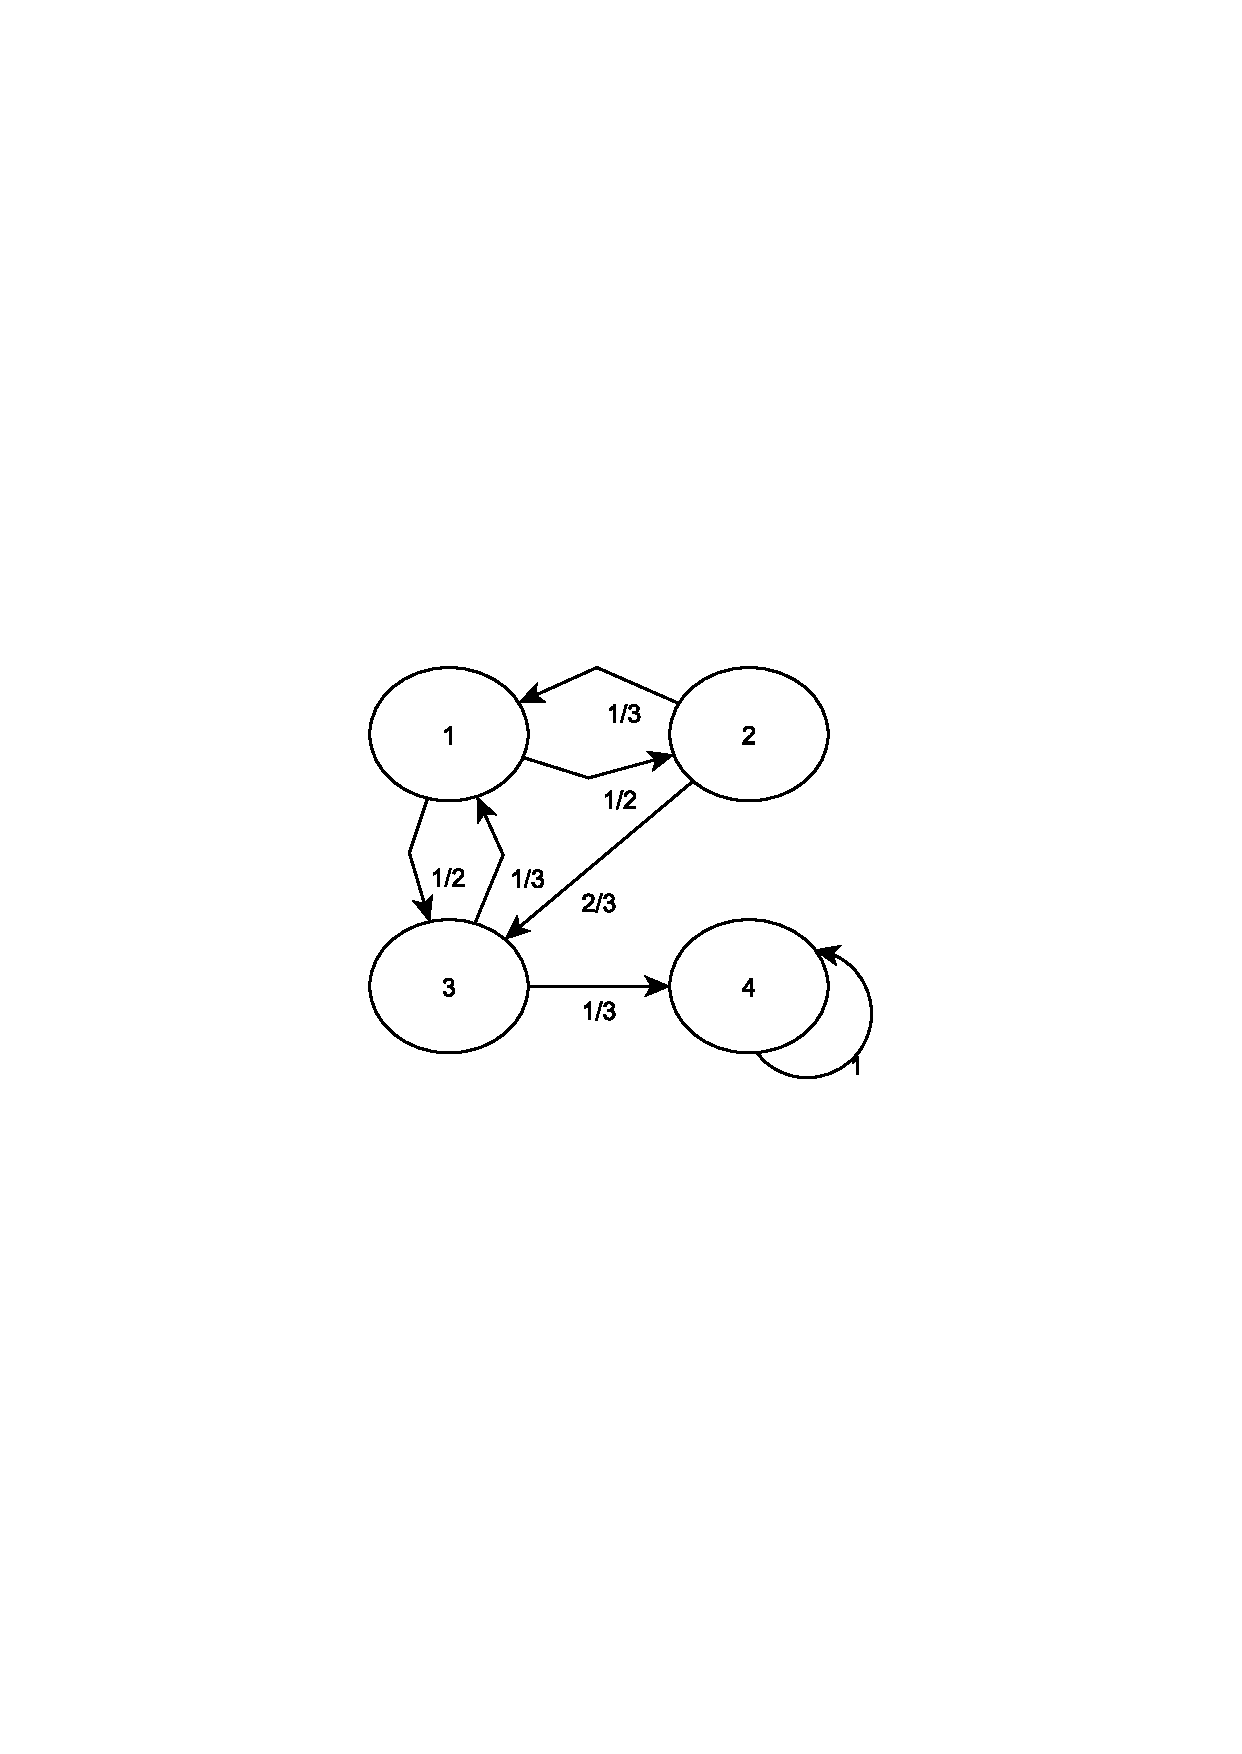
\includegraphics[scale=0.40]{cp_ex0_fig1.pdf}
\caption{Grafo delle transizioni}
\end{figure}

calcolare $p_{21}$.

\section{Svolgimento}

Al fine di calcolare $p_{21}$ modifico il grafo in modo tale da trasformare lo stato 1 in uno stato assorbente:

\begin{figure}[h]
\centering
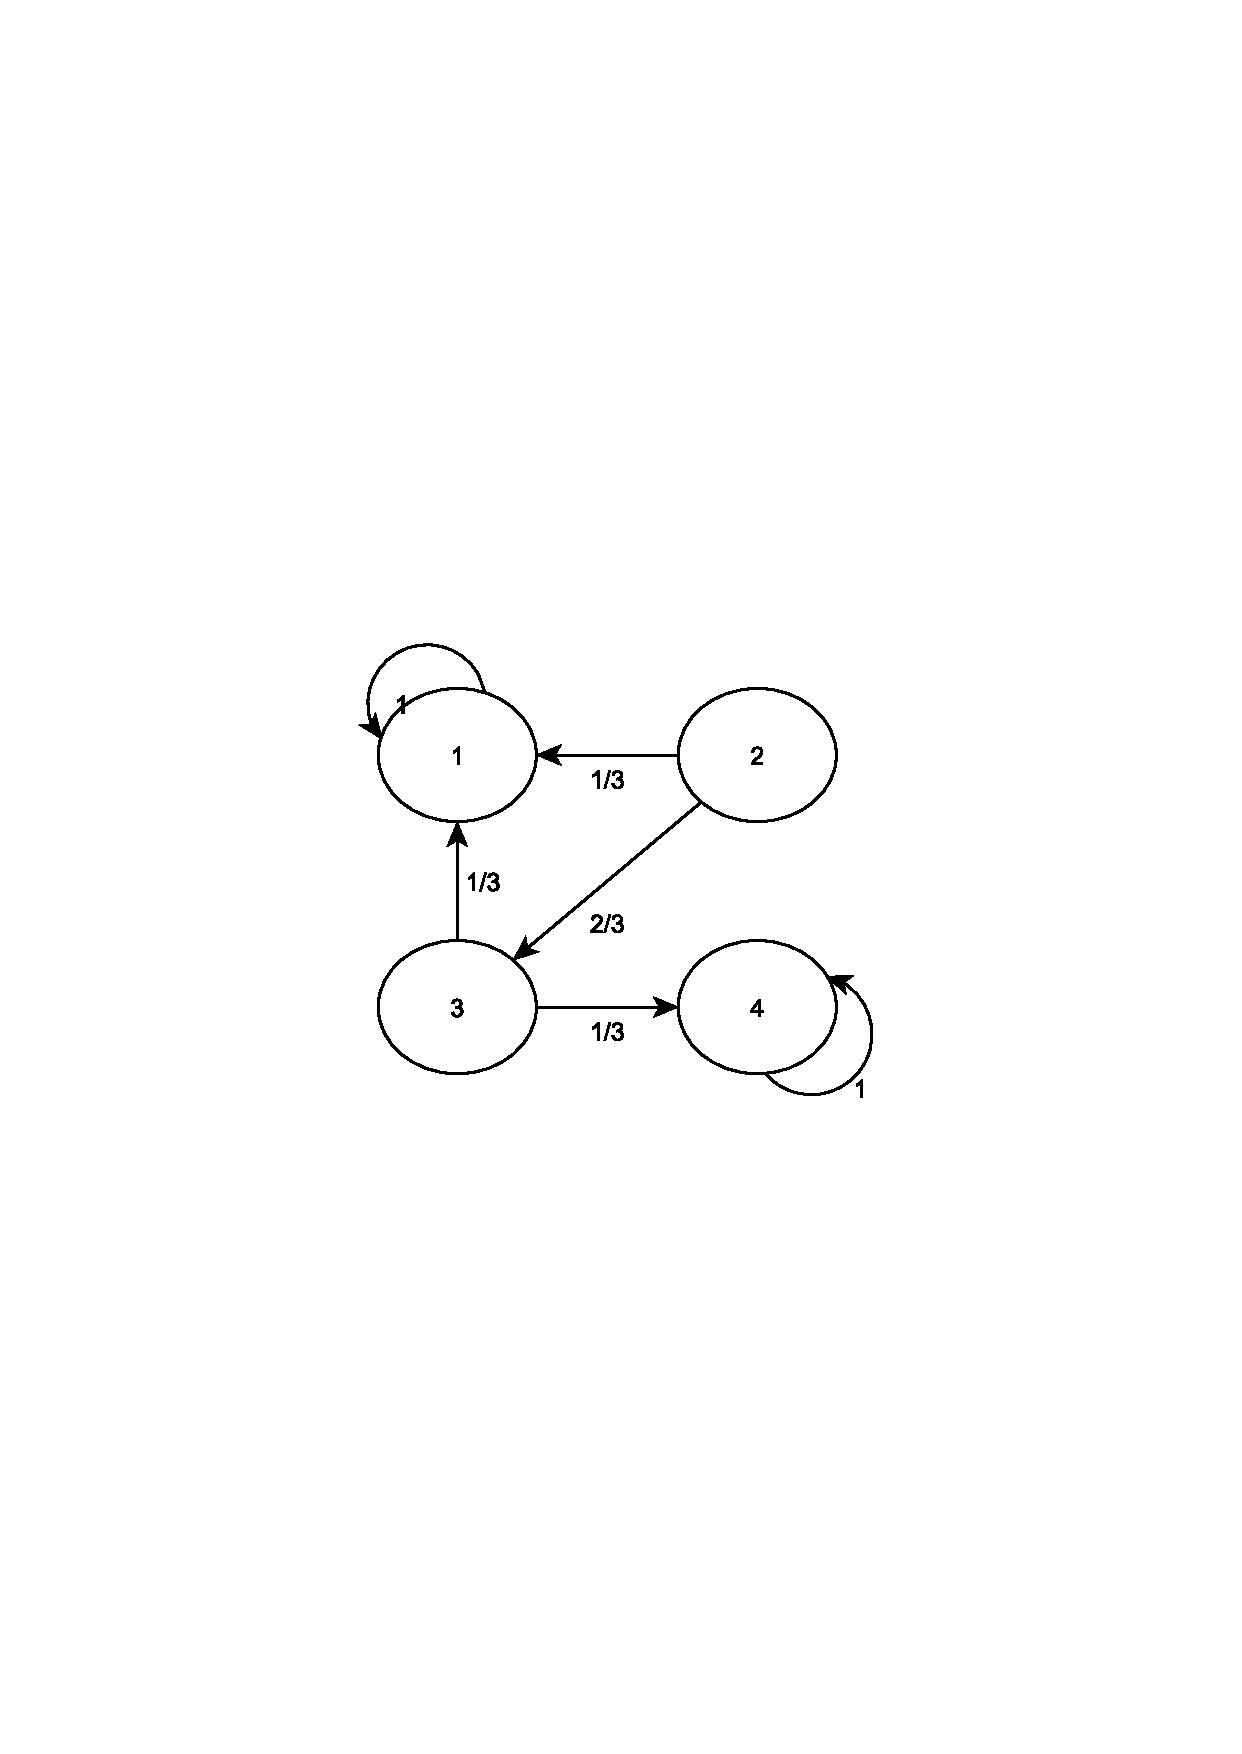
\includegraphics[scale=0.40]{cp_ex0_fig2.pdf}
\caption{Grafo delle transizioni modificato}
\end{figure}

Al fine di determinare la probabilit� di assorbimento dello stato $1$ ora possiamo usare la seguente formula:

$$
x_i = \sum_{j \in S \backslash T}{p_{i j}} + \sum_{j \in T}{p_{i j}x_j}, \forall i \in T
$$

Nel caso in esame l'insieme degli stati transienti risulta essere:

$$
T = \{ 2, 3 \}
$$

Otteniamo quindi un sistema di due equazioni:

$$
\begin{cases}
2 & x_2 = \frac{1}{3} + \frac{2}{3}x_3 \\
3 & x_3 = \frac{1}{3}                  \\
\end{cases}
$$

quindi $x_2 = \frac{5}{9}$ e $x_3 = \frac{1}{3}$. Concludendo si ha:

$$
\begin{cases}
x_2 & \lambda_2^{\{1\}}    \\
x_3 & \lambda_3^{\{1\}}     \\
\end{cases}
$$

\end{document}
